\begin{chapter}{Application}
    \label{chap:application}

    During its development process, the Restlessness framework has been tested on
    real deployed applications and this has been fundamental as it helped finding
    bugs and critical issues at an early stage.
    The main issues have emerged during the implementation of the backend for the
    project Spazio alla Scuola, a platform thought by the Fondazione Agnelli.

    The foundation is a non-profit, independent institute for social science research,
    born in 1966 in Turin, by the lawyer Agnelli, on the occasion of the centenary
    of the birth of the founder of Fiat, Senator Giovanni Agnelli.
    Its purpose is to work in support of scientific research and to disseminate
    knowledge of the conditions on which Italy's progress depends.

    The project Spazio alla Scuola aims to provide a concrete support to school
    leaders for lecture resumption on September 2020, given the health situation on the
    country due to the SARS-CoV-2 pandemic.
    The platform offers tools to verify capacity of classroom and other school spaces,
    to plan classrooms flows and staggering, in compliance with the distancing measures.
    The platform is provided as a free service and is available at the address
    \url{www.spazioallascuola.it} \cite{spazio_alla_scuola}.

    \section{Cold start}
    \label{subsec:cold_start}

    The first encountered problem has been Cold start, a new term in the serverless
    development that denotes the situation in which a serverless function is not
    active yet, so the platform must perform some resources initialization, with the
    main one being\footnote{Relatively to the Aws platform} \cite{aws_doc_runtimes}:

    \begin{itemize}
        \item Code: the project's code is uploaded in a zip archive, so it needs to
            be downloaded and extracted.
        \item Extensions: AWS allows to associate extensions to a lambda function, to
            integrate it with custom monitoring, security or other tools.
        \item Runtime: bootstrap operation for the chosen runtime environment,
            it is also possible to provide a custom runtime if needed.
        \item Function: code written by the developer, it can perform some resource
            initialization, such as creating a database connection.
    \end{itemize}

    \begin{figure}
        \centering
        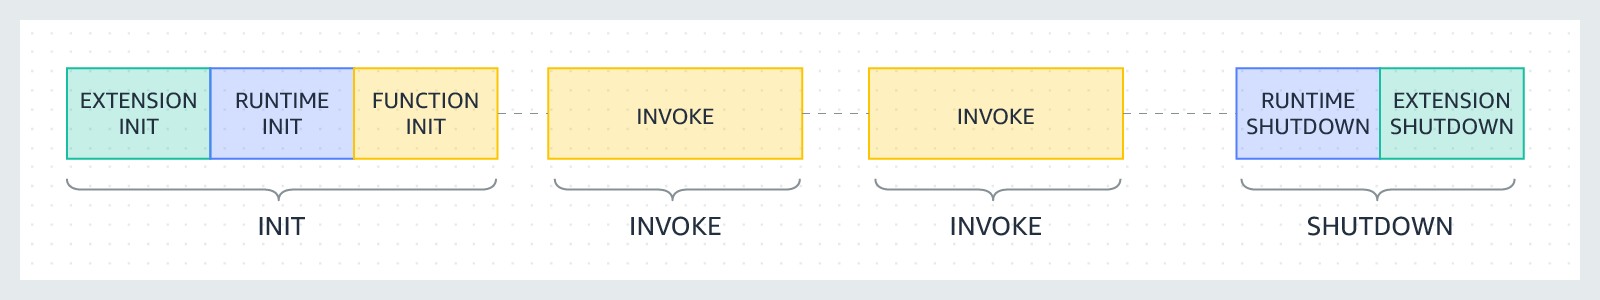
\includegraphics[width=\linewidth]{source/images/aws-lambda-lifecycle.png}
        \caption{Aws Lambda lifecycle}
        \label{fig:aws_lambda_lifecycle}
    \end{figure}

    The Cold start refers exactly to this Init phase and it represents an overhead to the
    function execution. However, once this phase is completed the function is ready,
    and subsequent invocations will not suffer from it. Then after some times without
    receiving any events, usually in the order of 5 to 20 minutes, the platform performs
    the Shutdown phase, so any following event causes the process to start again from
    the Init phase.
    For the majority of runtimes the duration of the Cold start varies in the order
    of tenths of a second, as shown on figure \ref{fig:cold_start_duration}. The provided
    numbers vary also based on the memory allocated for the function and the size of the
    provided code package.

    \begin{figure}
        \centering
        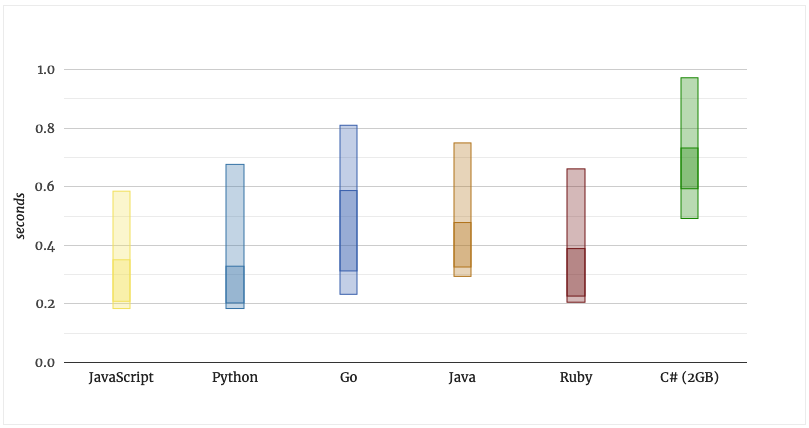
\includegraphics[width=\linewidth]{source/images/cold-start-duration.png}
        \caption{Cold start duration for different runtimes}
        \label{fig:cold_start_duration}
    \end{figure}

    In the particular case of the project Spazio alla Scuola the Cold start duration
    was experienced to be in the order of 1.5s, caused mainly from: mongodb
    initialization and connection (about 500ms) and third party libraries (about 400ms)
    and Restlessness overhead (about 50ms).

    One of the approaches to mitigate the effect of the Cold start proposed by the
    Serverless community has been the plugin named
    \href{https://www.npmjs.com/package/serverless-plugin-warmup}{serverless-plugin-warmup}.
    The plugin creates a scheduled function programmed to invoke the other defined functions,
    forcing the platform to keep an active container for each function.
    This way the Cold start effect remains present, but the end user of the api does
    not experience it.

    It has been decided to make this plugin an integral part of the Restlessness framework,
    granting out of the box support for it. From the Web Interface is possible to
    enabled or disable the warmup on the single endpoint, since not all functions may
    need it.
    By including the warmup plugin into the framework the effect of Cold start has
    been mitigated, however, it introduced another type of issue.

    \section{Database proxy}
    The project Spazio alla Scuola rely on the popular non relational database
    \href{https://www.mongodb.com}{mongodb}. As stated previously, each function
    run in its own runtime, independently from the others, consequently each function
    requiring database access needs to open a non shared connection.
    So the number of active connections can become quite high, depending on the number
    of active functions, furthermore, using mongodb the connection remains active for
    a certain amount of time even after the function has been shutdown.
    This leads to a high number of active connections, which is a problem, not only
    in terms of resources used, since each connection requires memory usage on the
    database, but also because mongodb has a limit of 500 concurrent connections,
    and once the threshold is exceeded the application experiences random errors when
    performing database operations.
    \begin{figure}
        \centering
        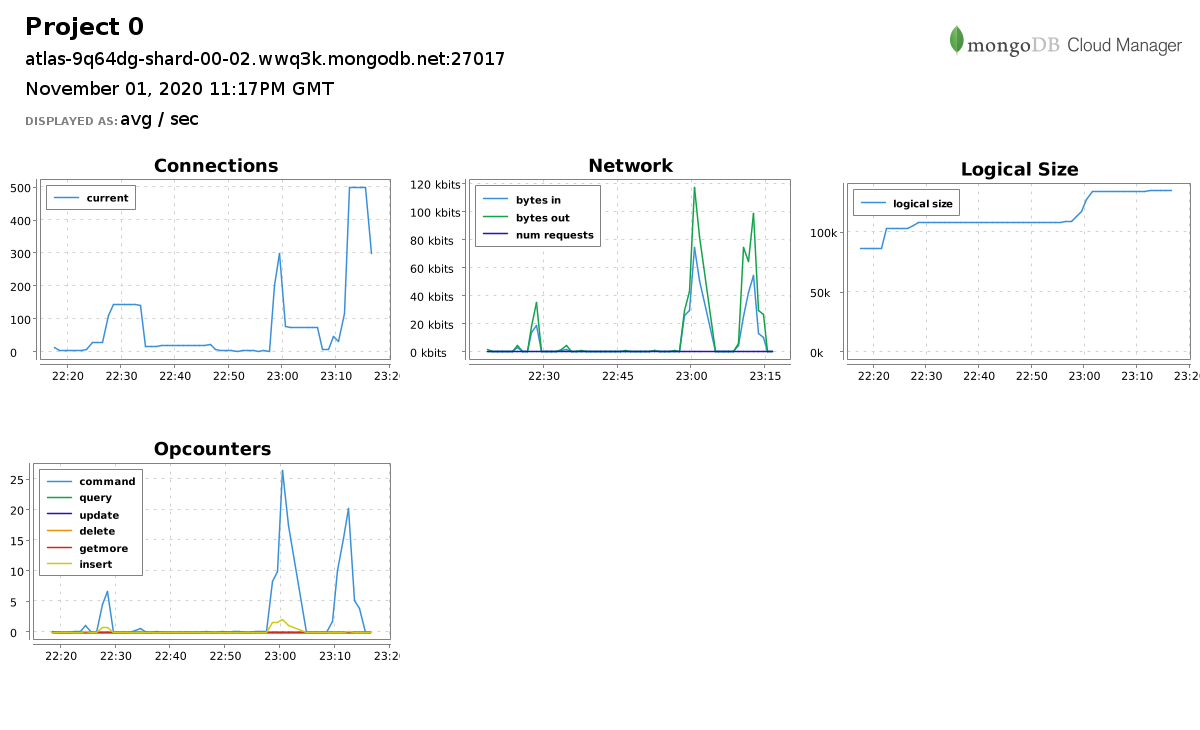
\includegraphics[width=7cm]{source/images/mongo-connections.png}
        \caption{Mongodb connections reaching the 500 threshold}
    \end{figure}

    Although the problem has been amplified by the introduction of the warmup plugin
    integration, it remains a critical issue for application that rely on the high
    scalability of the serverless platform.
    To address this problem on its relational databases, AWS rely on the usage of a
    proxy between the functions and the database. Exploiting the concept of a proxy,
    it has been decided to approach the problem in the same way, since a solution for
    for the mongo database does not exist at the moment.
    Restlessness already provides the package \textit{@restlessness/dao-mongo}, as
    described on section \ref{sec:data_access_object}, defining an abstraction level
    over the mongodb driver, so it was possible to include a proxy without changing
    the exposed methods for the users.
    It has been decided to develop an open source plugin, named
    \href{https://github.com/getapper/serverless-mongo-proxy}{serverless-mongo-proxy},
    to provide the proxy functionality, independently from the Restlessness framework,
    as shown on \ref{subsec:database_proxy}.
    The dao-mongo package then uses the plugin internally, providing an effective
    solution to the presented problem.

    \section{Micro services}
    \label{subsec:application_micro_services}
    During the deployment of an application on the AWS platform a number of resources
    are created for each function, to provides services such as logging, API Gateway
    for http events, permissions and others functionalities. The AWS platform has a
    threshold of maximum 200 resources definable for each service
    (\ref{subsec:sls_disadvantage}) and since for each function there are about 10
    resources associated, it follows that each service can define about 20 functions.
    Since the serverless paradigm proposes a Micro services oriented approach this
    limitation actually force developers to compose their application as a set of
    low complexity services.
    So the next step in the Restlessness framework development has been to switch
    between the management of a single service, to a multitude of services, under
    the same Restlessness project. With this approach it has been possible to split
    the functions of the project Spazio alla Scuola into multiple services, obtaining
    a more fine grained separation between its logic components.

    \bigbreak
    In conclusion the choice of using serverless, combined with the Restlessness
    framework for the backend api of Spazio alla Scuola, brought the desired benefits
    in terms of ease of development, after the proper framework improvements described
    previously. At its peak, the api service has managed 500 thousand requests,
    demonstrating the advantage of the natural scalability of the serverless approach.

\end{chapter}
